\let\negmedspace\undefined
\let\negthickspace\undefined
\documentclass[journal]{IEEEtran}
\usepackage[a5paper, margin=10mm, onecolumn]{geometry}
%\usepackage{lmodern} % Ensure lmodern is loaded for pdflatex
\usepackage{tfrupee} % Include tfrupee package

\setlength{\headheight}{1cm} % Set the height of the header box
\setlength{\headsep}{0mm}     % Set the distance between the header box and the top of the text

\usepackage{gvv-book}
\usepackage{gvv}
\usepackage{cite}
\usepackage{amsmath,amssymb,amsfonts,amsthm}
\usepackage{algorithmic}
\usepackage{graphicx}
\usepackage{textcomp}
\usepackage{xcolor}
\usepackage{txfonts}
\usepackage{listings}
\usepackage{enumitem}
\usepackage{mathtools}
\usepackage{gensymb}
\usepackage{comment}
\usepackage[breaklinks=true]{hyperref}
\usepackage{tkz-euclide} 
\usepackage{listings}
% \usepackage{gvv}                                        
\def\inputGnumericTable{}                                 
\usepackage[latin1]{inputenc}                                
\usepackage{color}                                            
\usepackage{array}                                            
\usepackage{longtable}                                       
\usepackage{calc}                                             
\usepackage{multirow}                                         
\usepackage{hhline}                                           
\usepackage{ifthen}                                           
\usepackage{lscape}
\begin{document}

\bibliographystyle{IEEEtran}
\vspace{3cm}

\title{4.2.19}
\author{EE24BTECH11012 - Bhavanisankar G S}
% \maketitle
% \newpage
% \bigskip
{\let\newpage\relax\maketitle}

\renewcommand{\thefigure}{\theenumi}
\renewcommand{\thetable}{\theenumi}
\setlength{\intextsep}{10pt} % Space between text and floats


\numberwithin{equation}{enumi}
\numberwithin{figure}{enumi}
\renewcommand{\thetable}{\theenumi}

\textbf{QUESTION} \\
Find the direction and normal vectors of the line $x+y=2$ . \\
\textbf{SOLUTION} \\

\begin{table}[h!]
	\centering
        \begin{tabular}[12pt]{|c|c|c|}
    \hline
    \textbf{Variable name} & \textbf{Description} & \textbf{Formula}\\ 
    \hline
		$A$ & $\myvec{2 \\ 3 \\ -4}$ &  \\
    \hline 
		$B$ & $\myvec{3 \\ -4 \\ -5}$ & \\
    \hline
		$C$ & $\myvec{3 \\ 2 \\ -3}$ &   \\
    \hline   
	$D$ & Distance of the point from the origin. &  $\abs{\vec{D}\myvec{a\\b\\c}}=\sqrt{a^2+b^2+c^2}$ = ? (\since \abs{D} is the distance of the point D from the origin . \\
	\hline
\end{tabular}


	\caption{Variables Used}
	\label{tab10.5.3.9.1}
\end{table} \\ \\ \\

\begin{align}
	y &= -x + 2 \\
	\leftrightarrow y &= mx + c \\
	A &= \myvec{1 \\ m} \\ 
	                 &= \myvec{1 \\ -1} \\
	B &= \myvec{ -m \\ 1 } \\
	              &= \myvec{ 1 \\ 1 } \\ 
\end{align}
where A and B denote the Direction and Normal vectors of the line respectively.

	\center{\boxed{A = \myvec{ 1 \\ -1}}} \\
	\center{\boxed{B = \myvec{ 1 \\ 1 }}} \\
	
\begin{figure}[h]
	\centering
	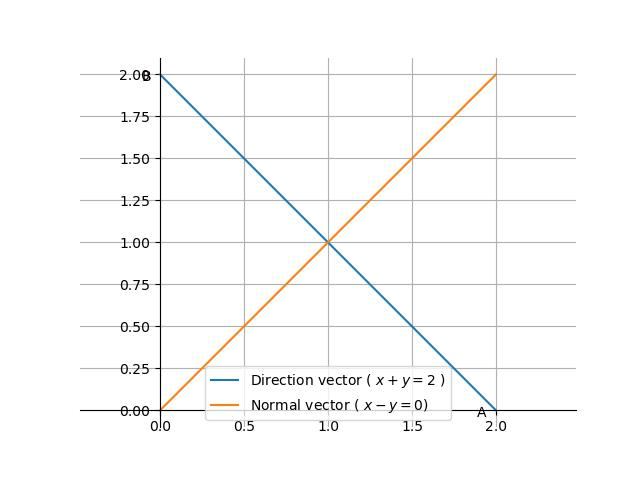
\includegraphics[width=0.8\textwidth]{figs/figure.jpg}
	\caption{A plot of the given question.}
\end{figure}
\end{document}
